% !TEX program = xelatex
% ============================================================
%  CivicPulse — Hackathon Technical Documentation
%  XeLaTeX source  |  Build: xelatex -interaction=nonstopmode civicpulse-docs.tex  (run twice)
%  Author: Ronit Sonawane
% ============================================================
\documentclass[11pt,a4paper]{article}

% ── Core packages ────────────────────────────────────────────
\usepackage{fontspec}
\usepackage[a4paper, top=2.2cm, bottom=2.4cm, left=2.5cm, right=2.5cm]{geometry}
\usepackage[table,dvipsnames]{xcolor}
\usepackage{graphicx}
\usepackage{longtable}
\usepackage{booktabs}
\usepackage{array}
\usepackage{tabularx}
\usepackage{multirow}
\usepackage{enumitem}
\usepackage{fancyhdr}
\usepackage{titlesec}
\usepackage{tcolorbox}
\usepackage{mdframed}
\usepackage{listings}
\usepackage{parskip}
\usepackage{microtype}
\usepackage{float}
\usepackage{caption}
\usepackage{subcaption}
\usepackage{tikz}
\usepackage{tikz-cd}
\usetikzlibrary{shapes.geometric,arrows.meta,positioning,fit,backgrounds,calc,shadows.blur}
\usepackage{lastpage}
\usepackage[hidelinks,
  pdftitle={CivicPulse: AI-Powered Civic Issue Reporting Platform},
  pdfauthor={Ronit Sonawane},
  pdfsubject={Hackathon Technical Documentation - Problem Statement 2: Community Hero},
  pdfkeywords={AI agents, LangGraph, Gemini, Google Cloud, civic tech, Next.js, India, DBSCAN, pgvector, PostGIS},
  pdfcreator={XeLaTeX with MiKTeX}
]{hyperref}
\usepackage{cleveref}

% ── Fonts ─────────────────────────────────────────────────────
\IfFontExistsTF{Segoe UI}{%
  \setsansfont{Segoe UI}[BoldFont={Segoe UI Bold},ItalicFont={Segoe UI Italic}]%
}{}
\IfFontExistsTF{Consolas}{%
  \setmonofont{Consolas}[Scale=0.88]%
}{}
\newfontfamily\marathifont{Nirmala UI}[Script=Devanagari]

% ── Colour Palette ────────────────────────────────────────────
\definecolor{cpblue}{HTML}{0D47A1}    % deep blue — headings
\definecolor{cpteal}{HTML}{00695C}    % teal — accents / section rules
\definecolor{cpgray}{HTML}{455A64}    % blue-grey — body subdued
\definecolor{cplight}{HTML}{E3F2FD}   % pale blue — callout bg
\definecolor{cpbg}{HTML}{EEF1F5}      % code bg — slightly darker
\definecolor{cpgreen}{HTML}{1B5E20}   % dark green — tip boxes
\definecolor{cporange}{HTML}{E65100}  % orange — warning boxes
\definecolor{cpred}{HTML}{B71C1C}     % dark red — caution
\definecolor{cpaccent}{HTML}{F59E0B}  % amber/gold — highlight badges
\definecolor{cpdark}{HTML}{0F172A}    % near-black — title page
\definecolor{rowalt}{HTML}{F5F7FA}    % table alternating row

% ── Section Heading Styles ────────────────────────────────────
\titleformat{\section}
  {\sffamily\color{cpblue}\LARGE\bfseries}
  {\makebox[0pt][r]{\color{cpteal}\rule[-2pt]{3.5pt}{16pt}\hspace{8pt}}\color{cpteal}\thesection}{0.8em}{}
  [\vspace{-2pt}\color{cpteal}\rule{\linewidth}{0.7pt}\vspace{4pt}]

\titleformat{\subsection}
  {\sffamily\color{cpblue}\large\bfseries}
  {\color{cpteal}\thesubsection}{0.7em}{}

\titleformat{\subsubsection}
  {\sffamily\color{cpteal}\normalsize\bfseries}
  {\thesubsubsection}{0.6em}{}

\titlespacing*{\section}{0pt}{22pt}{8pt}
\titlespacing*{\subsection}{0pt}{14pt}{5pt}

% ── tcolorbox Styles ─────────────────────────────────────────
\tcbuselibrary{skins,breakable}

\newtcolorbox{infobox}[1][]{
  enhanced, breakable,
  colback=cplight, colframe=cplight,
  borderline west={3.5pt}{0pt}{cpteal},
  sharp corners, boxrule=0pt,
  fonttitle=\sffamily\bfseries\small\color{cpteal},
  title={\textbf{ℹ\; Note}}, #1,
  left=8pt, right=8pt, top=6pt, bottom=6pt,
  drop shadow
}

\newtcolorbox{importantbox}[1][]{
  enhanced, breakable,
  colback=cpaccent!6, colframe=cpaccent!6,
  borderline west={3.5pt}{0pt}{cpaccent},
  sharp corners, boxrule=0pt,
  fonttitle=\sffamily\bfseries\small\color{cpaccent!80!black},
  title={\textbf{★\; Key Insight}}, #1,
  left=8pt, right=8pt, top=6pt, bottom=6pt,
  drop shadow
}

% ── Code listings ─────────────────────────────────────────────
\lstdefinestyle{civic}{
  backgroundcolor=\color{cpbg},
  basicstyle=\ttfamily\footnotesize,
  breaklines=true, breakatwhitespace=true,
  frame=l, framerule=2pt, rulecolor=\color{cpteal!40},
  xleftmargin=14pt, xrightmargin=10pt,
  aboveskip=8pt, belowskip=8pt,
  showstringspaces=false,
  keywordstyle=\color{cpblue}\bfseries,
  commentstyle=\color{cpgray}\itshape,
  stringstyle=\color{cpteal},
  numbers=left, numberstyle=\tiny\color{cpgray!50}, numbersep=6pt
}
\lstset{style=civic}

% ── Table helpers ─────────────────────────────────────────────
\newcolumntype{L}[1]{>{\raggedright\arraybackslash}p{#1}}
\newcolumntype{C}[1]{>{\centering\arraybackslash}p{#1}}
\newcommand{\thead}[1]{{\color{white}\bfseries\sffamily #1}}

% ── Header / footer ───────────────────────────────────────────
\pagestyle{fancy}
\fancyhf{}
\fancyhead[L]{\small\color{cpgray}\sffamily\textbf{CivicPulse} — Technical Documentation}
\fancyhead[R]{\small\color{cpgray}\sffamily\nouppercase{\leftmark}}
\fancyfoot[C]{\small\color{cpgray}\sffamily\thepage\;/\;\pageref{LastPage}}
\renewcommand{\headrulewidth}{0.4pt}
\renewcommand{\headrule}{\color{cpteal}\hrule width\headwidth height\headrulewidth}
\renewcommand{\footrulewidth}{0.15pt}
\renewcommand{\footrule}{{\color{cpteal!30}\hrule width\headwidth height\footrulewidth}\vspace{3pt}}

% ── Misc ──────────────────────────────────────────────────────
\captionsetup{font={small,sf}, labelfont={bf,color=cpblue}, skip=6pt}
\graphicspath{{document_assets/}}
\setlist[itemize]{leftmargin=*, topsep=3pt, itemsep=2pt}
\setlist[enumerate]{leftmargin=*, topsep=3pt, itemsep=2pt}
\renewcommand{\arraystretch}{1.3}
\setlength{\tabcolsep}{5pt}

% ── Convenience macros ────────────────────────────────────────
\newcommand{\tech}[1]{\texttt{\color{cpteal}#1}}
\newcommand{\file}[1]{\texttt{\footnotesize\color{cpgray}#1}}
\newcommand{\badge}[2]{\colorbox{#1}{\textcolor{white}{\tiny\bfseries #2}}}
\newcommand{\pilltag}[1]{%
  \tikz[baseline=(tag.base)]{\node[rounded corners=2pt, fill=cpblue!10,
    inner xsep=4pt, inner ysep=1.5pt, font=\tiny\sffamily\color{cpblue}] (tag) {#1};}%
}

% ── Screenshot frame command ──────────────────────────────────
\newcommand{\screenshot}[3][0.88\linewidth]{%
  \begin{figure}[H]
  \centering
  \begin{tcolorbox}[enhanced, colback=white, colframe=cpgray!20,
    boxrule=0.3pt, arc=4pt, boxsep=2pt,
    left=0pt, right=0pt, top=0pt, bottom=0pt,
    drop shadow, width=#1]
    \includegraphics[width=\linewidth]{#2}
  \end{tcolorbox}
  \vspace{-2pt}
  \caption{#3}
  \end{figure}
}

% ============================================================
\begin{document}
\sloppy

% ── COVER PAGE ───────────────────────────────────────────────
\begin{titlepage}
\begin{tikzpicture}[remember picture, overlay]
  % ── Gradient header ──
  \shade[top color=cpdark, bottom color=cpblue]
    (current page.north west) rectangle ([yshift=-10.5cm]current page.north east);
  % ── Decorative circles for depth ──
  \fill[white, opacity=0.04] ([xshift=3cm, yshift=-3cm]current page.north west) circle (2.5cm);
  \fill[white, opacity=0.03] ([xshift=14cm, yshift=-2cm]current page.north west) circle (1.8cm);
  \fill[white, opacity=0.05] ([xshift=9cm, yshift=-7.5cm]current page.north west) circle (1.2cm);
  \fill[white, opacity=0.03] ([xshift=17cm, yshift=-6.5cm]current page.north west) circle (2cm);
  % ── Accent stripe ──
  \fill[cpteal] ([yshift=-10.5cm]current page.north west) rectangle ([yshift=-10.8cm]current page.north east);
  % ── Bottom bar ──
  \fill[cpblue!8] (current page.south west) rectangle ([yshift=1.5cm]current page.south east);
  \draw[cpteal!30] ([yshift=1.5cm]current page.south west) -- ([yshift=1.5cm]current page.south east);
\end{tikzpicture}

% ── CP Monogram ──
\vspace*{0.3cm}

\begin{tikzpicture}[baseline]
  \node[circle, fill=white, minimum size=1.4cm, inner sep=0pt,
        drop shadow={shadow xshift=0.5mm, shadow yshift=-0.5mm, opacity=0.2}]
    {\color{cpblue}\fontsize{16}{16}\selectfont\sffamily\bfseries CP};
\end{tikzpicture}
\hspace{8pt}
{\color{white!70}\sffamily\small HACKATHON SUBMISSION}

\vspace{0.5cm}
{\color{white}\sffamily\bfseries\fontsize{42}{50}\selectfont CivicPulse}\\[6pt]
{\color{white!85}\sffamily\fontsize{16}{20}\selectfont AI-Powered Civic Issue Reporting Platform}\\[4pt]
{\color{white!60}\sffamily\small Problem Statement 2: Community Hero — Hyperlocal Problem Solver}

\vspace{0.7cm}

% ── Key Metrics Row ──
\begin{center}
\begin{tikzpicture}
  \node[rounded corners=4pt, draw=white!30, fill=white, fill opacity=0.15, text opacity=1, text=white,
        minimum width=2.9cm, minimum height=1.4cm, align=center] at (0,0)
    {\sffamily\fontsize{24}{28}\selectfont\bfseries 6\\[-3pt]{\footnotesize AI Agents}};
  \node[rounded corners=4pt, draw=white!30, fill=white, fill opacity=0.15, text opacity=1, text=white,
        minimum width=2.9cm, minimum height=1.4cm, align=center] at (3.5,0)
    {\sffamily\fontsize{24}{28}\selectfont\bfseries 14\\[-3pt]{\footnotesize API Endpoints}};
  \node[rounded corners=4pt, draw=white!30, fill=white, fill opacity=0.15, text opacity=1, text=white,
        minimum width=2.9cm, minimum height=1.4cm, align=center] at (7,0)
    {\sffamily\fontsize{20}{24}\selectfont\bfseries 3,300+\\[-3pt]{\footnotesize Lines of Code}};
  \node[rounded corners=4pt, draw=white!30, fill=white, fill opacity=0.15, text opacity=1, text=white,
        minimum width=2.9cm, minimum height=1.4cm, align=center] at (10.5,0)
    {\sffamily\fontsize{24}{28}\selectfont\bfseries 9\\[-3pt]{\footnotesize Google Services}};
\end{tikzpicture}
\end{center}

\vspace{1.0cm}

% ── Metadata Card ──
\begin{tcolorbox}[
  enhanced, colback=white, colframe=cpgray!20,
  boxrule=0.4pt, arc=5pt,
  borderline west={3pt}{0pt}{cpteal},
  left=12pt, right=12pt, top=10pt, bottom=10pt,
  drop shadow
]
\sffamily
\begin{tabular}{@{}L{3.8cm} L{10cm}@{}}
  \textbf{\color{cpblue}Submitted by}  & Ronit Sonawane \\
  \textbf{\color{cpblue}Affiliation}   & B.Tech 1st Year, Computer Science \& Engineering, IIT Guwahati \\
  \textbf{\color{cpblue}Team Size}     & Solo (Individual Submission) \\
  \textbf{\color{cpblue}Repository}    & \href{https://github.com/ronits2407/civicpulse}{\tech{github.com/ronits2407/civicpulse}} \\
  \textbf{\color{cpblue}Live App}      & \href{https://civicpulse-948264080742.asia-south1.run.app}{\tech{civicpulse-948264080742.asia-south1.run.app}} \\
  \textbf{\color{cpblue}Deployment}    & Google Cloud Run \textbf{(asia-south1)} \\
  \textbf{\color{cpblue}Date}          & June 2026 \\
\end{tabular}
\end{tcolorbox}

\vspace{0.6cm}

% ── Abstract (pull-quote style) ──
\begin{tcolorbox}[
  enhanced, breakable,
  colback=white, colframe=white,
  borderline west={3pt}{0pt}{cpteal},
  sharp corners, boxrule=0pt,
  left=10pt, right=10pt, top=6pt, bottom=6pt
]
\textbf{\color{cpteal}\sffamily Abstract.} CivicPulse is a full-stack, AI-powered civic issue reporting platform designed for Indian cities. Citizens report infrastructure, sanitation, safety, utility, and environmental problems via text, photo, video, or voice. A six-agent LangGraph pipeline powered by Google Gemini 2.5 Flash and Pro automatically classifies, deduplicates, validates, generates resolution briefs, and predicts future civic hotspots. The platform is deployed live on Google Cloud Run with a complete CI/CD pipeline using GitHub Actions and Workload Identity Federation. It supports any typed language via automatic translation, community verification with quorum-based voting, karma gamification, TSP-optimised field team routing, and a fully featured admin dashboard.
\end{tcolorbox}

\vspace*{\fill}

% ── Tech pills ──
\begin{center}
\pilltag{Gemini 2.5 Flash/Pro}\;\pilltag{LangGraph}\;\pilltag{Next.js 16}\;\pilltag{Supabase PostGIS+pgvector}\;\pilltag{Cloud Run}\;\pilltag{Mapbox GL}
\end{center}
\vspace{0.3cm}
\end{titlepage}
\thispagestyle{empty}
\setcounter{page}{1}

% ── TABLE OF CONTENTS ─────────────────────────────────────────
\tableofcontents
\clearpage

% ── PROJECT HIGHLIGHTS ────────────────────────────────────────
\begin{tcolorbox}[
  enhanced, breakable,
  colback=cpteal!4, colframe=cpteal!4,
  borderline west={3.5pt}{0pt}{cpteal},
  sharp corners, boxrule=0pt,
  left=8pt, right=8pt, top=8pt, bottom=8pt,
  drop shadow
]
{\sffamily\bfseries\color{cpteal}\large Project Highlights}
\vspace{4pt}
\begin{itemize}[leftmargin=1.2em, itemsep=3pt]
  \item \textbf{Solo submission} by a 1st-year B.Tech student at IIT Guwahati
  \item \textbf{6 AI agents} orchestrated by LangGraph with conditional branching and retry/resume
  \item \textbf{3-layer deduplication:} pgvector cosine similarity + PostGIS spatial + Gemini semantic verification
  \item \textbf{Any typed language supported} via automatic detection and translation (Agent 0)
  \item \textbf{TSP-optimised routing} for municipal field teams via Google Maps Routes API
  \item \textbf{Deployed live} on Google Cloud Run with zero-credential CI/CD (Workload Identity Federation)
  \item \textbf{Community verification} with quorum-based voting and karma gamification
  \item \textbf{Predictive hotspot analysis} using geographic DBSCAN clustering + Gemini 2.5 Pro
\end{itemize}
\end{tcolorbox}
\vspace{6pt}

% ── §0 EVALUATION CRITERIA QUICK REFERENCE ───────────────────
\section*{Evaluation Criteria Quick Reference}
\addcontentsline{toc}{section}{Evaluation Criteria Quick Reference}
\label{sec:eval}

\begin{importantbox}
Judges: each row maps a scoring criterion to the sections where evidence is presented. This table is intentionally placed \textbf{before} the main content for fast navigation.
\end{importantbox}

\vspace{6pt}
\begin{tabularx}{\linewidth}{@{} L{4.5cm} C{1.8cm} X @{}}
\toprule
\rowcolor{cpblue}
\thead{Criterion} & \thead{Weight} & \thead{Key Sections} \\
\midrule
Problem Solving \& Impact   & 20\% & §\ref{sec:problem} (Problem), §\ref{sec:solution} (Solution), §\ref{sec:ux} (User Story) \\
Agentic Depth               & 20\% & §\ref{sec:agents} (All 6 agents, conditional edges, retry mechanism) \\
Innovation \& Creativity    & 20\% & §\ref{sec:innovation} (Dual-AI, 3-layer dedup, gamification, TSP routing, tunnel automation) \\
Google Technologies         & 15\% & §\ref{sec:google} (Gemini Flash/Pro/Embedding, Maps Geocoding/Routes, Cloud Run, WIF, OAuth) \\
Product Experience \& Design& 10\% & §\ref{sec:design} (Screenshots, mobile-first design, GitHub-style UI) \\
Technical Implementation    & 10\% & §\ref{sec:technical} (AI client, auth flow, community verification, WKB decoding) \\
Completeness \& Usability   & 5\%  & §\ref{sec:completeness} (End-to-end flows, tests, health check) \\
\bottomrule
\end{tabularx}

\clearpage

% ============================================================
\section{Problem Statement and Motivation}
\label{sec:problem}
% ============================================================

\subsection{The Challenge}

\begin{mdframed}[linecolor=cpblue!40, linewidth=0.6pt, innerleftmargin=10pt, innerrightmargin=10pt,
  innertopmargin=6pt, innerbottommargin=6pt, backgroundcolor=cplight]
\textit{``Build a platform that enables citizens to identify, report, validate, track, and resolve community issues through collaboration, data, and intelligent automation. The solution should encourage transparency, accountability, and community participation.''}
\end{mdframed}

\subsection{Why This Matters}

India has over \textbf{4,000 urban local bodies} serving 500 million urban citizens. Existing civic grievance redressal systems suffer from systemic failures:

\begin{itemize}
  \item \textbf{Fragmented reporting:} Citizens navigate different portals, phone lines, or offices per issue type. No unified platform exists.
  \item \textbf{No intelligent triage:} A life-threatening open manhole and a faded road marking enter the same queue with identical priority.
  \item \textbf{Duplicate flooding:} The same pothole is reported 50 times. Each becomes a separate ticket, wasting municipal bandwidth.
  \item \textbf{Zero accountability:} Once filed, citizens have no visibility into whether their report was acknowledged or assigned.
  \item \textbf{Language barriers:} India has 22 scheduled languages. English-only platforms exclude the majority of citizens.
  \item \textbf{No predictive capability:} Municipalities are purely reactive — fixing potholes after accidents, clearing drains after flooding.
\end{itemize}

\subsection{How CivicPulse Addresses Every Aspect}

\begin{tabularx}{\linewidth}{@{} L{4.2cm} X @{}}
\toprule
\rowcolor{cpblue}
\thead{Problem} & \thead{CivicPulse Solution} \\
\midrule
Fragmented reporting     & Single platform: text, photo, video, GPS, and voice — all in one submission \\
No intelligent triage    & 6-agent AI pipeline: classifies, deduplicates, validates, generates SLA deadlines \\
Duplicate flooding       & 3-layer: pgvector cosine similarity + PostGIS spatial search + AI semantic verification \\
Zero accountability      & Real-time pipeline tracking via Supabase Realtime WebSocket subscriptions \\
Language barriers        & Agent 0 automatically detects and translates typed reports in any language to English \\
No predictive capability & Agent 5: geographic DBSCAN clustering + Gemini 2.5 Pro for predictive hotspot analysis \\
Lack of engagement       & Karma gamification, leaderboard, community verification, shareable Impact Receipts \\
\bottomrule
\end{tabularx}

\clearpage

% ============================================================
\section{Solution Overview}
\label{sec:solution}
% ============================================================

CivicPulse is a full-stack AI-powered civic reporting and resolution platform. It accepts reports through multiple modalities, processes them through a six-agent LangGraph pipeline, and provides both citizens and municipal administrators with real-time visibility into every stage of the issue lifecycle.

\subsection{High-Level System Architecture}

\begin{figure}[H]
\centering
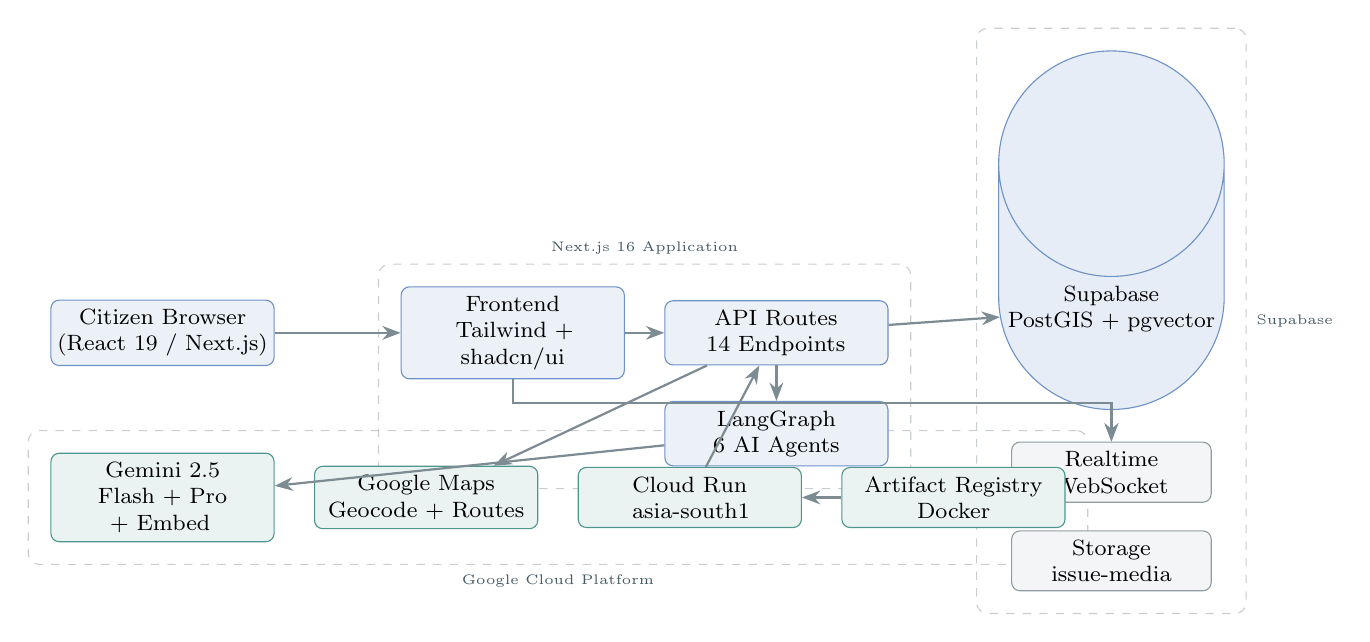
\begin{tikzpicture}[
  node distance=0.6cm and 0.5cm,
  box/.style={rounded corners=3pt, draw=cpblue!60, fill=cpblue!8, minimum height=0.75cm,
              text width=2.6cm, align=center, font=\footnotesize},
  gcp/.style={rounded corners=3pt, draw=cpteal!70, fill=cpteal!8, minimum height=0.75cm,
              text width=2.6cm, align=center, font=\footnotesize},
  ext/.style={rounded corners=3pt, draw=cpgray!60, fill=cpgray!6, minimum height=0.75cm,
              text width=2.3cm, align=center, font=\footnotesize},
  db/.style={cylinder, shape border rotate=90, draw=cpblue!60, fill=cpblue!10,
             minimum height=1cm, minimum width=2.2cm, align=center, font=\footnotesize},
  arr/.style={-Stealth, thick, color=cpgray!70},
  grp/.style={draw=cpgray!30, dashed, rounded corners=4pt, fill=none, inner sep=8pt}
]

% ── Citizens ──────────────────────────────────────────────────
\node[box] (citizen) {Citizen Browser\\\footnotesize(React 19 / Next.js)};

% ── Application ───────────────────────────────────────────────
\node[box, right=1.6cm of citizen] (fe) {Frontend\\\footnotesize Tailwind + shadcn/ui};
\node[box, right=0.5cm of fe] (api) {API Routes\\\footnotesize 14 Endpoints};
\node[box, below=0.45cm of api] (pipe) {LangGraph\\\footnotesize 6 AI Agents};

% ── Supabase ──────────────────────────────────────────────────
\node[db, right=1.4cm of api, yshift=0.3cm] (db) {Supabase\\\footnotesize PostGIS + pgvector};
\node[ext, below=0.4cm of db] (rt) {Realtime\\\footnotesize WebSocket};
\node[ext, below=0.35cm of rt] (store) {Storage\\\footnotesize issue-media};

% ── GCP ───────────────────────────────────────────────────────
\node[gcp, below=1.1cm of citizen] (gemini) {Gemini 2.5\\\footnotesize Flash + Pro + Embed};
\node[gcp, right=0.5cm of gemini] (maps) {Google Maps\\\footnotesize Geocode + Routes};
\node[gcp, right=0.5cm of maps] (cr) {Cloud Run\\\footnotesize asia-south1};
\node[gcp, right=0.5cm of cr] (ar) {Artifact Registry\\\footnotesize Docker};

% ── Arrows ────────────────────────────────────────────────────
\draw[arr] (citizen) -- (fe);
\draw[arr] (fe) -- (api);
\draw[arr] (api) -- (pipe);
\draw[arr] (api) -- (db);
\draw[arr] (pipe) -- (gemini);
\draw[arr] (api) -- (maps);
\draw[arr] (db) -- (rt);
\draw[arr] (cr) -- (api);
\draw[arr] (ar) -- (cr);
\draw[arr] (fe.south) -- ++(0,-0.3) -| (rt.north);

% ── Group boxes ───────────────────────────────────────────────
\begin{scope}[on background layer]
  \node[grp, fit=(fe)(api)(pipe), label={[font=\tiny\color{cpgray}]above:Next.js 16 Application}] {};
  \node[grp, fit=(db)(rt)(store), label={[font=\tiny\color{cpgray}]right:Supabase}] {};
  \node[grp, fit=(gemini)(maps)(cr)(ar), label={[font=\tiny\color{cpgray}]below:Google Cloud Platform}] {};
\end{scope}
\end{tikzpicture}
\caption{High-level system architecture: citizen browser through Next.js application to GCP and Supabase}
\end{figure}

\subsection{Landing Page}

\screenshot[0.88\linewidth]{s1_landing.jpg}{CivicPulse landing page — role selection for citizens and municipal administrators}

% ============================================================
\section{System Architecture}
\label{sec:arch}
% ============================================================

\subsection{Technology Stack}

\begin{longtable}{@{} L{3cm} L{4cm} L{2.2cm} L{5.4cm} @{}}
\toprule
\rowcolor{cpblue}
\thead{Layer} & \thead{Technology} & \thead{Version} & \thead{Purpose} \\
\midrule
\endhead
Framework          & Next.js App Router    & 16.2.9  & Full-stack React with Turbopack \\
Language           & TypeScript            & 5.x     & Type-safe strict-mode development \\
Runtime            & Bun                   & Latest  & Package management \& scripting \\
UI Library         & shadcn/ui (Radix+Mira)& 4.11.0  & Accessible composable components \\
Styling            & Tailwind CSS          & 4.x     & Utility-first CSS \\
Animation          & Framer Motion         & 12.41.0 & Transitions \& micro-interactions \\
Maps               & Mapbox GL JS          & 3.25.0  & Interactive map rendering \\
AI (Primary)       & Google Gemini         & 2.10.0  & Flash/Pro for all 6 agents \\
AI (Alternate)     & OpenAI SDK (Ollama)   & 6.45.0  & Self-hosted model support \\
Agent Orchestration& LangGraph             & 1.4.6   & StateGraph with conditional edges \\
Database           & Supabase (PostgreSQL 17) & —    & PostGIS + pgvector data store \\
Auth               & Supabase Auth         & —       & Google OAuth + Email magic link \\
Geocoding          & Google Maps Geocoding & —       & Reverse geocoding (lat/lng → address) \\
Routing            & Google Maps Routes API& —       & TSP-optimised field team routing \\
Weather            & Open-Meteo API        & —       & Historical weather data (free, no key) \\
Clustering         & Geographic DBSCAN (custom) & — & Haversine-based district-constrained \\
Geo Parsing        & wkx                   & 0.5.0   & PostGIS WKB/WKT geometry decoding \\
Deployment         & Google Cloud Run      & —       & Serverless container hosting \\
CI/CD              & GitHub Actions        & —       & Automated build \& deploy pipeline \\
Container          & Docker (multi-stage)  & —       & node:20-alpine production image \\
\bottomrule
\end{longtable}

\clearpage

% ============================================================
\section{Agentic AI Pipeline — Deep Dive}
\label{sec:agents}
% ============================================================

The core of CivicPulse is a \textbf{six-agent pipeline} orchestrated by LangGraph. Each agent is a discrete node in a \tech{StateGraph} reading from and writing to a shared \tech{AgentState}. The pipeline uses conditional edges to short-circuit at any stage.

\subsection{Pipeline Architecture}

\begin{figure}[H]
\centering
\begin{tikzpicture}[
  node distance=0.5cm,
  agent/.style={rounded corners=4pt, draw=cpblue!60, fill=cpblue!7,
                minimum width=3.8cm, minimum height=1cm,
                align=center, font=\small},
  terminal/.style={rounded corners=12pt, draw=cpteal!70, fill=cpteal!10,
                   minimum width=3.8cm, minimum height=0.7cm,
                   align=center, font=\small\bfseries},
  sidenode/.style={rounded corners=4pt, draw=cpgray!50, fill=cpgray!6,
                   minimum width=2.6cm, minimum height=0.75cm,
                   align=center, font=\footnotesize},
  arr/.style={-Stealth, thick, cpgray!70},
  darr/.style={-Stealth, thick, cpgray!40, dashed},
  labarr/.style={font=\tiny\itshape\color{cpgray}}
]
\node[terminal] (start) {Citizen Submits Report};
\node[agent, below=0.5cm of start] (a0) {\textbf{Agent 0: Translation}\\{\footnotesize Gemini Flash · Language detect + translate}};
\node[agent, below=0.5cm of a0] (a1) {\textbf{Agent 1: Classifier}\\{\footnotesize Gemini Flash + Vision · Category / Severity}};
\node[agent, below=0.5cm of a1] (a2) {\textbf{Agent 2: Deduplication}\\{\footnotesize pgvector + PostGIS + AI · 3 layers}};
\node[agent, below=0.5cm of a2] (a3) {\textbf{Agent 3: Validation}\\{\footnotesize Open-Meteo + Gemini Flash · Credibility score}};
\node[agent, below=0.5cm of a3] (a4) {\textbf{Agent 4: Resolution}\\{\footnotesize Gemini Flash · Civic brief + SLA deadline}};
\node[terminal, below=0.5cm of a4] (save) {Save to Supabase DB};
\node[terminal, below=0.3cm of save] (rt) {Realtime Push to Dashboard};

% Side path — async Agent 5
\node[sidenode, right=1.8cm of a3] (a5) {\textbf{Agent 5}\\{\footnotesize Gemini Pro}\\{\footnotesize Predictive}};

% Arrows
\draw[arr] (start) -- (a0);
\draw[arr] (a0) -- node[labarr,right]{success} (a1);
\draw[arr] (a1) -- node[labarr,right]{not duplicate} (a2);
\draw[arr] (a2) -- node[labarr,right]{score ≥ 6} (a3);
\draw[arr] (a3) -- node[labarr,right]{always} (a4);
\draw[arr] (a4) -- (save);
\draw[arr] (save) -- (rt);

% Error / short-circuit paths
\draw[darr] (a0.east) -- ++(1.2,0) |- node[labarr,right,pos=0.2]{on error} (save.east);
\draw[darr] (a2.west) -- ++(-1.2,0) |- node[labarr,left,pos=0.2]{duplicate found} (save.west);
\draw[darr] (a3.east) ++(0,-0.2) -- ++(0.8,0) |- node[labarr,right,pos=0.15]{score < 6 → community review} (save.east);

% Agent 5 async
\draw[darr] (a5.south) -- ++(0,-0.5) -| (save.east);
\node[font=\tiny\itshape\color{cpgray}, right=0.2cm of a5] {admin-triggered};
\end{tikzpicture}
\caption{LangGraph StateGraph pipeline with conditional edges and Agent 5 async path}
\end{figure}

\subsection{Pipeline Stage Tracking}

Every issue has a \tech{pipeline\_stage} column updated in real time. The citizen dashboard subscribes via Supabase Realtime and renders a visual progress stepper.

\begin{tabular}{@{} L{5.5cm} L{8.5cm} @{}}
\toprule
\rowcolor{cpblue}
\thead{Stage Value} & \thead{Meaning} \\
\midrule
\tech{agent0\_translation}         & Language detection in progress \\
\tech{agent1\_classifier}          & Classification in progress \\
\tech{agent2\_deduplication}       & Duplicate check in progress \\
\tech{agent3\_validation}          & Credibility scoring in progress \\
\tech{agent4\_resolution}          & Civic brief generation in progress \\
\tech{completed}                   & Full pipeline completed successfully \\
\tech{awaiting\_community\_review} & Credibility $<$ 6; awaiting citizen votes \\
\tech{review\_rejected}            & Community voted to reject the report \\
\tech{*\_failed}                   & Agent failed; eligible for retry/resume \\
\bottomrule
\end{tabular}

\subsection{Agent 0: Translation}
\label{sec:agent0}
\textbf{File:} \file{lib/agents/agent0-translation.ts}

Detects the language of a citizen's typed report and translates it to English so all downstream agents operate on a common language. Gemini Flash returns structured JSON: \tech{\{detected\_language, translated\_text, thought\_process\}}. The original language and translation trace are stored for audit purposes. This means a citizen typing in Marathi, Tamil, or Bengali receives identical AI processing quality as one typing in English.

\begin{infobox}
\textbf{Voice input note:} The browser's Web Speech API (\tech{webkitSpeechRecognition}) recognises speech in \textbf{English} (en-US) only — it does not reliably transcribe Indian regional languages. Citizens who speak Marathi, Hindi, or Tamil should \textit{type} their report; Agent 0 will then detect and translate automatically. A toast notification in the UI informs users if their browser does not support voice input at all.
\end{infobox}

\subsection{Agent 1: Classifier}
\label{sec:agent1}
\textbf{File:} \file{lib/agents/agent1-classifier.ts}

\textbf{Multimodal classification:} If an image is attached, the agent first downloads it, optimises via \tech{sharp} (1024px, JPEG 85\%), and sends it as base64 inline data to Gemini Flash Vision. The visual description is combined with the (translated) text and sent for classification.

\textbf{Output fields:} \tech{category} (one of: infrastructure, sanitation, safety, utility, environment), \tech{subcategory}, \tech{severity} (1–10), \tech{is\_emergency} (boolean), \tech{suggested\_title}, \tech{department\_id} (matched from the \tech{departments} table by category scope).

\subsection{Agent 2: Deduplication — Three-Layer Strategy}
\label{sec:agent2}
\textbf{File:} \file{lib/agents/agent2-deduplication.ts}

\begin{figure}[H]
\centering
\begin{tikzpicture}[
  box/.style={rounded corners=3pt, draw=cpblue!60, fill=cpblue!7, text width=3cm,
              minimum height=0.8cm, align=center, font=\footnotesize},
  decision/.style={diamond, draw=cpteal!70, fill=cpteal!8, text width=1.8cm,
                   minimum height=0.7cm, align=center, font=\tiny},
  result/.style={rounded corners=8pt, draw=cpgray!50, fill=cpgray!6,
                 text width=3cm, minimum height=0.7cm, align=center, font=\footnotesize},
  arr/.style={-Stealth, thick, cpgray!60},
  node distance=0.45cm
]
\node[box] (new) {New Issue Report};
\node[box, below=0.4cm of new] (l1) {Layer 1: pgvector\\\footnotesize cosine similarity ≥ 0.85};
\node[decision, below=0.4cm of l1] (c1) {Match?};
\node[box, right=1.6cm of c1] (ai1) {AI Semantic\\\footnotesize Verification};
\node[box, below=0.5cm of c1] (l2) {Layer 2: PostGIS\\\footnotesize ST\_DWithin 200m + category};
\node[decision, below=0.4cm of l2] (c2) {Match?};
\node[box, right=1.6cm of c2] (ai2) {AI Semantic\\\footnotesize Verification};
\node[result, below=0.5cm of c2] (unique) {Unique → Agent 3};
\node[result, right=1.5cm of ai1, yshift=-0.5cm] (dup) {Duplicate → cluster\\\footnotesize + close report};
\draw[arr] (new)--(l1); \draw[arr] (l1)--(c1);
\draw[arr] (c1) -- node[font=\tiny,above]{Yes} (ai1);
\draw[arr] (c1) -- node[font=\tiny,right]{No} (l2);
\draw[arr] (l2)--(c2);
\draw[arr] (c2) -- node[font=\tiny,above]{Yes} (ai2);
\draw[arr] (c2) -- node[font=\tiny,right]{No} (unique);
\draw[arr] (ai1) -- node[font=\tiny,right]{confirmed} (dup);
\draw[arr] (ai2) -- node[font=\tiny,right]{confirmed} (dup);
\draw[arr] (ai1.south) -- ++(0,-0.3) -| (l2.east);
\draw[arr] (ai2.south) -- ++(0,-0.3) -| (unique.east);
\end{tikzpicture}
\caption{Agent 2 three-layer deduplication: vector similarity → spatial proximity → AI semantic verification}
\end{figure}

\textbf{Why three layers:} Vector similarity alone produces false positives (similar language, different locations). Spatial proximity alone misses differently worded reports. AI verification is the final semantic judge — ``Traffic light broken at MG Road'' vs ``Pothole near MG Road signal'' are correctly identified as \textit{different} issues despite overlapping in both vector space and geography.

\subsection{Agent 3: Validation}
\label{sec:agent3}
\textbf{File:} \file{lib/agents/agent3-validation.ts}

Two-loop reasoning:
\begin{enumerate}
  \item \textbf{Weather relevance check:} Asks Gemini if the issue type needs weather context (waterlogging = yes; broken streetlight = no).
  \item \textbf{Conditional weather fetch:} If required, fetches live data from Open-Meteo (temperature, precipitation, wind) — free, no API key.
  \item \textbf{Credibility assessment:} Gemini scores the report 1–10 considering: weather consistency, description verifiability, severity proportionality, and spam signals.
  \item \textbf{Routing:} Score $\geq 6$ → Agent 4. Score $< 6$ → community review queue with push notification to nearby citizens.
\end{enumerate}

\subsection{Agent 4: Resolution}
\label{sec:agent4}
\textbf{File:} \file{lib/agents/agent4-resolution.ts}

\textbf{SLA matrix:}
\begin{tabular}{@{} L{3.2cm} C{2.4cm} C{2.4cm} C{2.4cm} @{}}
\toprule
\rowcolor{cpblue}
\thead{Category} & \thead{High (7\textendash 10)} & \thead{Medium (4\textendash 6)} & \thead{Low (1\textendash 3)} \\
\midrule
Infrastructure & 24 h & 72 h & 168 h \\
Sanitation     & 12 h & 48 h & 96 h  \\
Safety         & 6 h  & 24 h & 72 h  \\
Utility        & 12 h & 48 h & 96 h  \\
Environment    & 48 h & 120 h & 240 h \\
\bottomrule
\end{tabular}

Generates a 150–200 word professional civic action brief. If the original language is non-English, also generates a \tech{local\_civic\_brief} translated into the citizen's language.

\subsection{Agent 5: Predictive Intelligence}
\label{sec:agent5}
\textbf{File:} \file{lib/agents/agent5-predictive.ts}

Admin-triggered predictive analysis powered by \textbf{Gemini 2.5 Pro}:
\begin{enumerate}
  \item Fetches issues within a configurable lookback period (30/60/90 days).
  \item Decodes PostGIS WKB location strings via \tech{wkx}.
  \item Runs \textbf{geographic DBSCAN clustering} (\file{lib/utils/clustering.ts}) on coordinates using \textbf{Haversine distance} — clusters are constrained to a maximum 50 km radius (≈ one Indian district). The number of clusters is fully data-driven with no fixed upper limit; geographically distant cities always form separate clusters.
  \item For each cluster, summarises historical issues (category, severity, dates) and prompts Gemini 2.5 Pro for forward-looking predictions.
  \item Stores results in \tech{predictive\_alerts} (PostGIS POINT centroid, confidence 0–1, \tech{basis\_summary}).
  \item Displayed as a heatmap overlay in the admin dashboard.
\end{enumerate}

\begin{importantbox}
\textbf{Why geographic DBSCAN over K-Means:} The previous approach used K-Means with Euclidean lat/lng distance, which treats 1° of longitude the same as 1° of latitude — a significant distortion at India's latitudes. Additionally K-Means required a fixed cluster count (capped at 10), causing Mumbai and Pune (360 km apart) to merge into one cluster. The current algorithm uses Haversine distance in metres with a 50 km district-level cap, producing geographically accurate, data-driven clusters without any fixed limit.
\end{importantbox}

\subsection{LangGraph StateGraph Wiring}
\textbf{File:} \file{lib/agents/pipeline.ts}

The pipeline uses LangGraph's \tech{StateGraph} with 16 typed channels in \tech{AgentState}: \tech{reportId, rawText, originalLanguage, englishTranslation, translationTrace, imageUrl, videoUrl, coordinates, userId, classification, deduplication, validation, resolution, error, imageAnalysis, address}.

\textbf{Background execution:} The pipeline is invoked via Next.js 16's \tech{after()} — it runs asynchronously after the HTTP response is returned. The \file{/api/reports/process} endpoint returns immediately with the \tech{issueId} while agents process in the background.

\textbf{Pipeline retry/resume:} If any agent fails (LLM timeout, network error), the issue's \tech{pipeline\_stage} is set to \tech{*\_failed}. The \file{/api/reports/retry} endpoint reconstructs the full \tech{AgentState} from database columns and resumes from the failed agent — not from the beginning.

\clearpage

% ============================================================
\section{Google Technologies Used}
\label{sec:google}
% ============================================================

\subsection{Gemini 2.5 Flash — Agents 0 through 4}
Every agent uses \tech{generateStructuredJSON<T>()} with \tech{temperature: 0.1} for deterministic output. Each agent has a carefully crafted system prompt constraining the model to valid JSON only, no markdown, no preamble.

\subsection{Gemini 2.5 Pro — Agent 5}
Reserved exclusively for predictive analysis. The \tech{usePro} flag in the unified AI client switches from \tech{gemini-2.5-flash} to \tech{gemini-2.5-pro}. This is reserved for complex multi-step reasoning where accuracy matters more than latency.

\subsection{Gemini Embedding (gemini-embedding-001)}
Generates 768-dimensional embeddings in two places: (1) on report submission for storage in the \tech{issues.embedding} pgvector column, and (2) at Agent 2 runtime for vector similarity comparison. \tech{outputDimensionality: 768} is set explicitly to match the pgvector column.

\subsection{Gemini Flash Vision — Agent 1}
Photos uploaded with reports are analysed via Gemini's multimodal API. Images are first optimised by \tech{sharp} (1024px max, JPEG 85\%) then sent as base64 inline data. This provides visual evidence for classification: a photo of a broken streetlight yields ``Damaged pole with exposed wiring — safety hazard on residential road,'' which is combined with the text description for more accurate severity scoring.

\subsection{Google Maps Geocoding API}
\textbf{File:} \file{app/api/geocode/route.ts}. Reverse-geocodes GPS coordinates into human-readable addresses by parsing \tech{address\_components} from the Maps API for \tech{locality} (city) and \tech{administrative\_area\_level\_1} (state). Returns a clean ``City, State'' string in real time as the citizen selects a location.

\subsection{Google Maps Routes API — TSP Optimisation}
\textbf{File:} \file{app/api/admin/routes/optimize/route.ts}. Accepts an origin point and issue waypoints and calls \tech{computeRoutes} with \tech{optimizeWaypointOrder: true}, solving the Travelling Salesman Problem for minimal total travel distance. Returns the optimised order, total duration/distance, and an encoded polyline for Mapbox rendering.

\subsection{Google Cloud Run — asia-south1}
\begin{itemize}
  \item \textbf{Region:} asia-south1 (Mumbai) for low latency to Indian users
  \item \textbf{Live URL:} \href{https://civicpulse-948264080742.asia-south1.run.app}{\tech{https://civicpulse-948264080742.asia-south1.run.app}}
  \item \textbf{Configuration:} \tech{--allow-unauthenticated}; environment variables via \tech{cloudrun-env.yaml}; port 3000; non-root container user
\end{itemize}

\subsection{Google Artifact Registry}
Docker images tagged with Git SHA pushed to \tech{asia-south1-docker.pkg.dev/\allowbreak civicpulse-500507/\allowbreak civicpulse-repo/\allowbreak civicpulse}.

\subsection{Workload Identity Federation}
The CI/CD pipeline authenticates to GCP with \textbf{zero stored credentials} — GitHub's OIDC token is exchanged for a short-lived GCP access token. Pool: \tech{projects/948264080742/locations/global/workloadIdentityPools/github-pool}. No service account JSON keys stored anywhere.

\subsection{Google OAuth}
Supabase Auth is configured with the Google OAuth provider (\tech{NEXT\_PUBLIC\_GOOGLE\_CLIENT\_ID}). The callback at \file{app/auth/callback/route.ts} exchanges the code for a session and reads a \tech{role} query parameter to route admins to \file{/admin/dashboard}.

\clearpage

% ============================================================
\section{Innovation and Creativity}
\label{sec:innovation}
% ============================================================

\subsection{Dual-Provider AI Architecture}
A single environment variable (\tech{AI\_PROVIDER=gemini} or \tech{ollama}) switches the entire AI backend. The unified client (\file{lib/ai/client.ts}) abstracts over both providers:

\begin{tabular}{@{} L{3.5cm} L{4.5cm} L{4.5cm} @{}}
\toprule
\rowcolor{cpblue}
\thead{Feature} & \thead{Gemini (Default)} & \thead{Ollama (Alternate)} \\
\midrule
Flash model     & \tech{gemini-2.5-flash}   & \tech{qwen3:30b-a3b} \\
Pro model       & \tech{gemini-2.5-pro}     & \tech{qwen3:235b-a22b} \\
Vision model    & \tech{gemini-2.5-flash}   & \tech{llava} \\
Embedding model & \tech{gemini-embedding-001} & \tech{nomic-embed-text} \\
\bottomrule
\end{tabular}

This enables development without burning API credits and demonstrates vendor-agnostic architecture.

\subsection{Cloudflared Tunnel for Hybrid AI}
\textbf{File:} \file{scripts/manage-gcloud.ps1}

Solves the problem of routing Cloud Run traffic through a local GPU running Ollama:
\begin{enumerate}
  \item Starts \tech{cloudflared tunnel --url http://localhost:11434} in background.
  \item Parses the assigned temporary HTTPS URL from the log.
  \item Updates \tech{.env.production} and pushes to GitHub Secrets via \tech{gh secret set}.
  \item Triggers a new Cloud Run deployment automatically.
\end{enumerate}
One command connects a developer's local GPU to a globally deployed cloud application.

\subsection{Three-Layer Deduplication}
No existing civic platform combines vector similarity, spatial proximity, and semantic AI verification. Each layer catches cases the others miss — see §\ref{sec:agent2} for details.

\subsection{Universal Language Support (Agent 0)}
India's linguistic diversity is a major barrier for civic engagement. CivicPulse breaks this barrier by running all inputs through \textbf{Agent 0}, which automatically detects the input language and translates it into English before it enters the main LangGraph pipeline. It supports \textit{any} language supported by Gemini. When the pipeline resolves, the final civic brief and status updates are translated back into the citizen's original language in the dashboard.

\subsection{Predictive Hotspot Clustering (DBSCAN)}
To identify emerging civic hotspots before they escalate, CivicPulse uses a custom geographic DBSCAN (Density-Based Spatial Clustering of Applications with Noise) algorithm. This is calculated directly in \file{lib/utils/clustering.ts} using the Haversine formula to account for the Earth's curvature.

\begin{figure}[H]
\centering
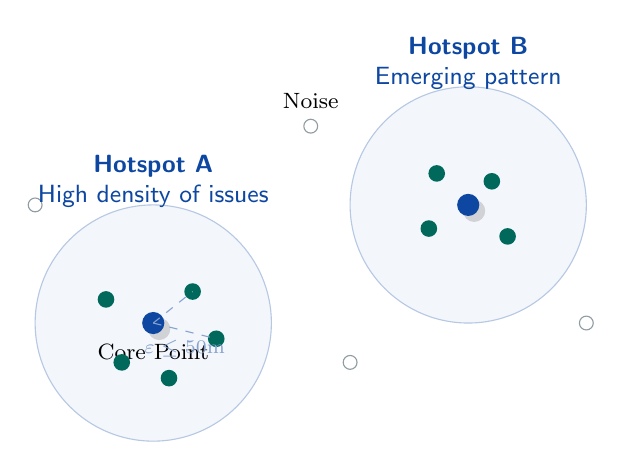
\begin{tikzpicture}[
    dot/.style={circle, fill=cpteal, inner sep=0pt, minimum size=6pt},
    noise/.style={circle, draw=cpgray!60, fill=white, inner sep=0pt, minimum size=5pt},
    core/.style={circle, fill=cpblue, inner sep=0pt, minimum size=8pt, drop shadow={opacity=0.3}},
    halo/.style={circle, draw=cpblue!30, fill=cpblue!5, inner sep=0pt, minimum size=3cm}
  ]
  % Cluster 1
  \node[halo] at (0,0) {};
  \node[core, label=below:{\footnotesize Core Point}] at (0,0) {};
  \node[dot] at (0.5, 0.4) {};
  \node[dot] at (-0.6, 0.3) {};
  \node[dot] at (0.2, -0.7) {};
  \node[dot] at (-0.4, -0.5) {};
  \node[dot] at (0.8, -0.2) {};
  
  % Cluster 2
  \node[halo] at (4, 1.5) {};
  \node[core] at (4, 1.5) {};
  \node[dot] at (4.3, 1.8) {};
  \node[dot] at (3.6, 1.9) {};
  \node[dot] at (4.5, 1.1) {};
  \node[dot] at (3.5, 1.2) {};
  
  % Noise points
  \node[noise, label=above:{\footnotesize Noise}] at (2, 2.5) {};
  \node[noise] at (2.5, -0.5) {};
  \node[noise] at (-1.5, 1.5) {};
  \node[noise] at (5.5, 0) {};
  
  % Connecting lines for epsilon neighborhood
  \draw[dashed, cpblue!50] (0,0) -- (0.5, 0.4);
  \draw[dashed, cpblue!50] (0,0) -- (0.8, -0.2) node[midway, below, font=\scriptsize\color{cpblue}] {$\varepsilon \le 50$m};
  
  % Annotations
  \node[font=\sffamily\small\color{cpblue}, align=center] at (0, 1.8) {\textbf{Hotspot A}\\High density of issues};
  \node[font=\sffamily\small\color{cpblue}, align=center] at (4, 3.3) {\textbf{Hotspot B}\\Emerging pattern};
\end{tikzpicture}
\caption{DBSCAN algorithm categorises closely grouped civic issues into actionable hotspots, while filtering out isolated noise incidents.}
\end{figure}

The algorithm identifies dense regions of issues (Core Points) within an $\varepsilon$-radius, groups them, and passes the aggregate data to Agent 5 (Gemini 2.5 Pro) to generate predictive maintenance alerts.

\subsection{Karma Gamification}

\begin{tabular}{@{} L{6cm} C{2cm} L{5cm} @{}}
\toprule
\rowcolor{cpblue}
\thead{Event} & \thead{Points} & \thead{Rationale} \\
\midrule
Report an issue                  & +10 & Incentivise reporting \\
Participate in community review  & +2  & Incentivise verification \\
Vote with the majority           & +5  & Reward accurate judgment \\
Report confirmed by community    & +20 & Reward legitimate reports \\
Issue resolved by municipality   & +50 & Celebrate civic impact \\
Report rejected by community     & --5 & Penalise spam/false reports \\
\bottomrule
\end{tabular}

\subsection{Impact Receipt}
When an issue is resolved, citizens generate a shareable OG image (1200×630px) via \tech{next/og} showing: issue title, location, fix time, estimated citizens affected, and CivicPulse branding — designed for WhatsApp and social media sharing.

\subsection{Community Verification with Quorum}
Issues with credibility $< 6$ enter \tech{community\_review}. Nearby citizens vote verify/deny. Quorum rules: minimum 3 votes; if confirms $\geq$ denies the issue resumes the pipeline at Agent 4. If denies $>$ confirms the issue is closed and the reporter loses 5 karma. The vote endpoint internally calls \file{/api/reports/retry} on confirmation.

\subsection{Route Optimisation with TSP}
The admin Route Planner clusters open issues geographically and computes an optimal visit sequence for municipal field teams via Google Maps Routes API \tech{optimizeWaypointOrder: true}. The encoded polyline is rendered on a Mapbox map.

\clearpage

% ============================================================
\section{Product Experience and Design}
\label{sec:design}
% ============================================================

\subsection{Design Philosophy}

CivicPulse follows a \textbf{GitHub-inspired design system}: high information density, functional colour usage, and zero decorative elements. The philosophy: a civic platform used daily by municipal workers must prioritise clarity over aesthetics.

\begin{itemize}
  \item \textbf{Dark mode by default:} \tech{\#0d1117} background, \tech{\#c9d1d9} text, \tech{\#161b22} cards, \tech{\#30363d} borders — exactly GitHub's dark palette.
  \item \textbf{Functional colours:} Green (\tech{\#2da44e}) for success; Blue (\tech{\#0969da}) for primary actions; Red (\tech{\#cf222e}) for emergencies. No decorative gradients.
  \item \textbf{Inter font} via \tech{next/font/google} — clean, legible, widely supported.
  \item \textbf{shadcn/ui (Radix primitives)} for keyboard navigation and ARIA accessibility.
\end{itemize}

\subsection{Mobile-First Responsive Design}

CivicPulse is built with a \textbf{mobile-first approach} — every screen is designed for a 375px handset viewport first and enhanced for wider screens. This is deliberate: the typical Indian citizen reporting a pothole is holding a smartphone, not sitting at a desktop.

\begin{itemize}
  \item \textbf{Fluid layouts:} Tailwind's \tech{sm:}, \tech{md:}, \tech{lg:} breakpoints provide seamless adaptation from 320px feature phones to 1920px admin monitors.
  \item \textbf{Touch targets:} All interactive elements meet the WCAG 44×44px minimum tap target size.
  \item \textbf{Report page on mobile:} Text area fills the screen; GPS, camera, and image upload are one-tap actions designed for outdoor use without fine motor precision.
  \item \textbf{Dashboard on mobile:} Issue cards collapse by default, expanding on tap; pipeline stepper is horizontally scrollable; mini-map opens as a full-screen overlay.
  \item \textbf{Admin dashboard on mobile:} The full admin inbox, map, Agent 5 panel, and Route Planner all reflow to single-column layouts on small screens — tested across multiple viewport widths.
  \item \textbf{Dark OLED mode:} The \tech{\#0d1117} background reduces power consumption significantly on AMOLED/OLED phone displays, extending battery life during field use.
  \item \textbf{PWA-ready:} A service worker stub (\file{public/sw.js}) and web manifest are in place for future offline support and home-screen installation.
\end{itemize}

\subsection{Key Screens}

\screenshot[0.85\linewidth]{s2_login.jpg}{Login — Google OAuth + email magic link}

\screenshot[0.85\linewidth]{s3_report_top.jpg}{Report page — text input + voice button}

\clearpage

\screenshot[0.85\linewidth]{s4_report_bottom.jpg}{Report page — image upload, webcam, GPS map}

\screenshot[0.85\linewidth]{s5_dashboard.jpg}{Citizen dashboard — issue cards with pipeline stepper}

\clearpage

\begin{figure}[H]
\centering
\begin{subfigure}[t]{0.45\linewidth}
  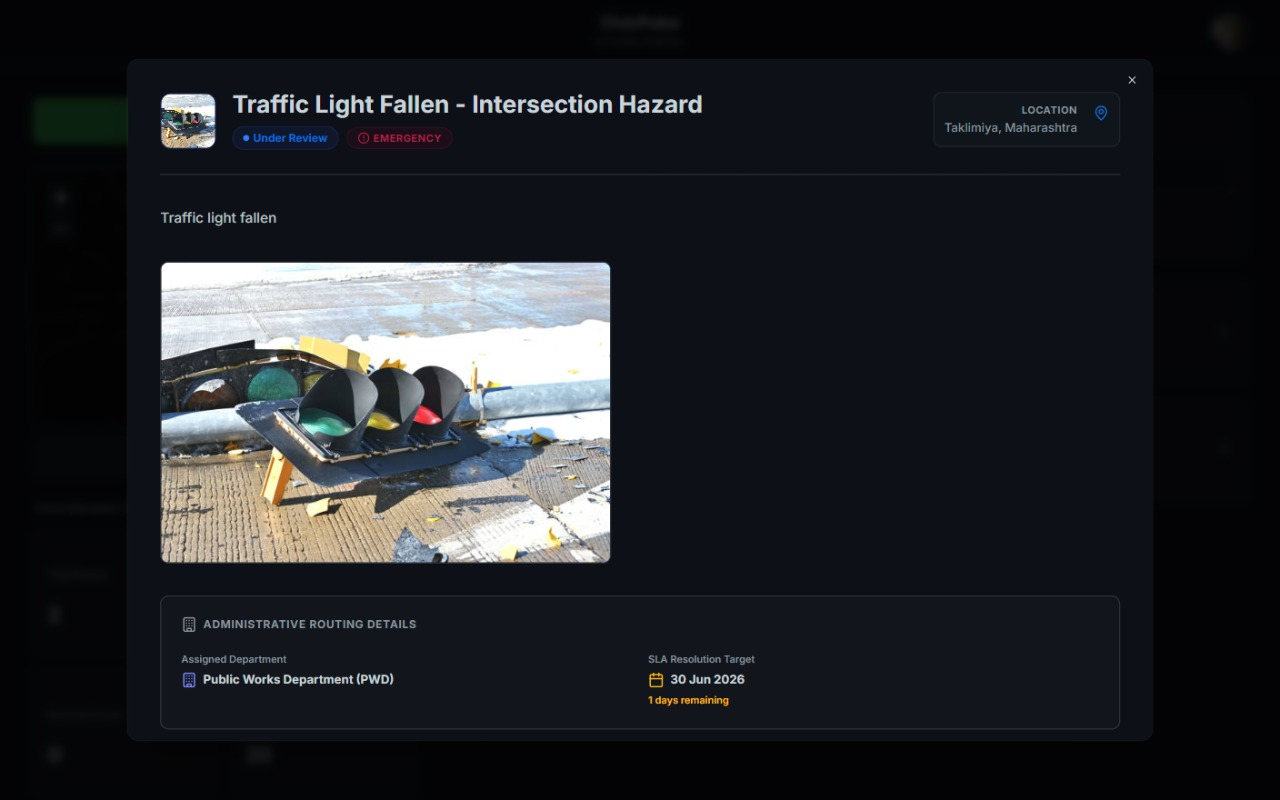
\includegraphics[width=\linewidth]{s6_issue_detail_1.jpg}
  \caption{Pipeline 1}
\end{subfigure}\hfill
\begin{subfigure}[t]{0.45\linewidth}
  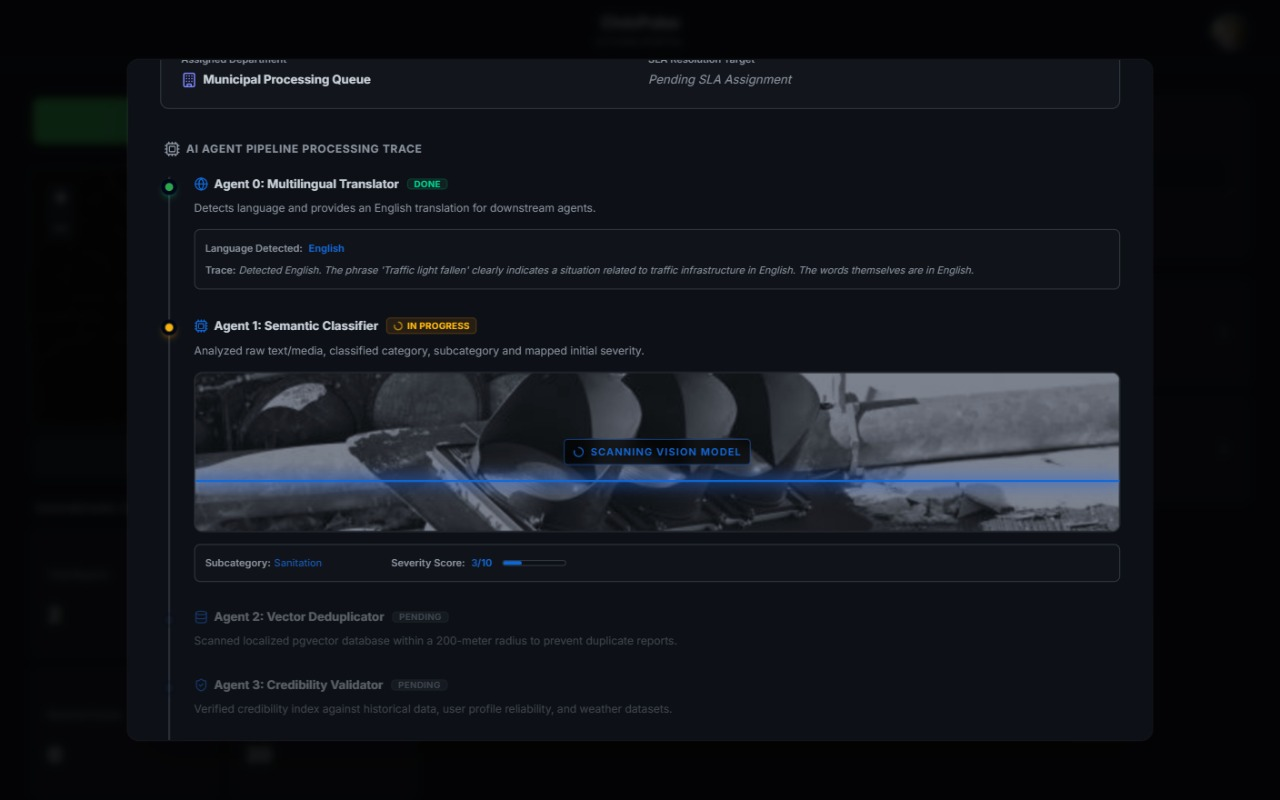
\includegraphics[width=\linewidth]{s6_issue_detail_2.jpg}
  \caption{Pipeline 2}
\end{subfigure}
\end{figure}

\begin{figure}[H]
\centering
\begin{subfigure}[t]{0.45\linewidth}
  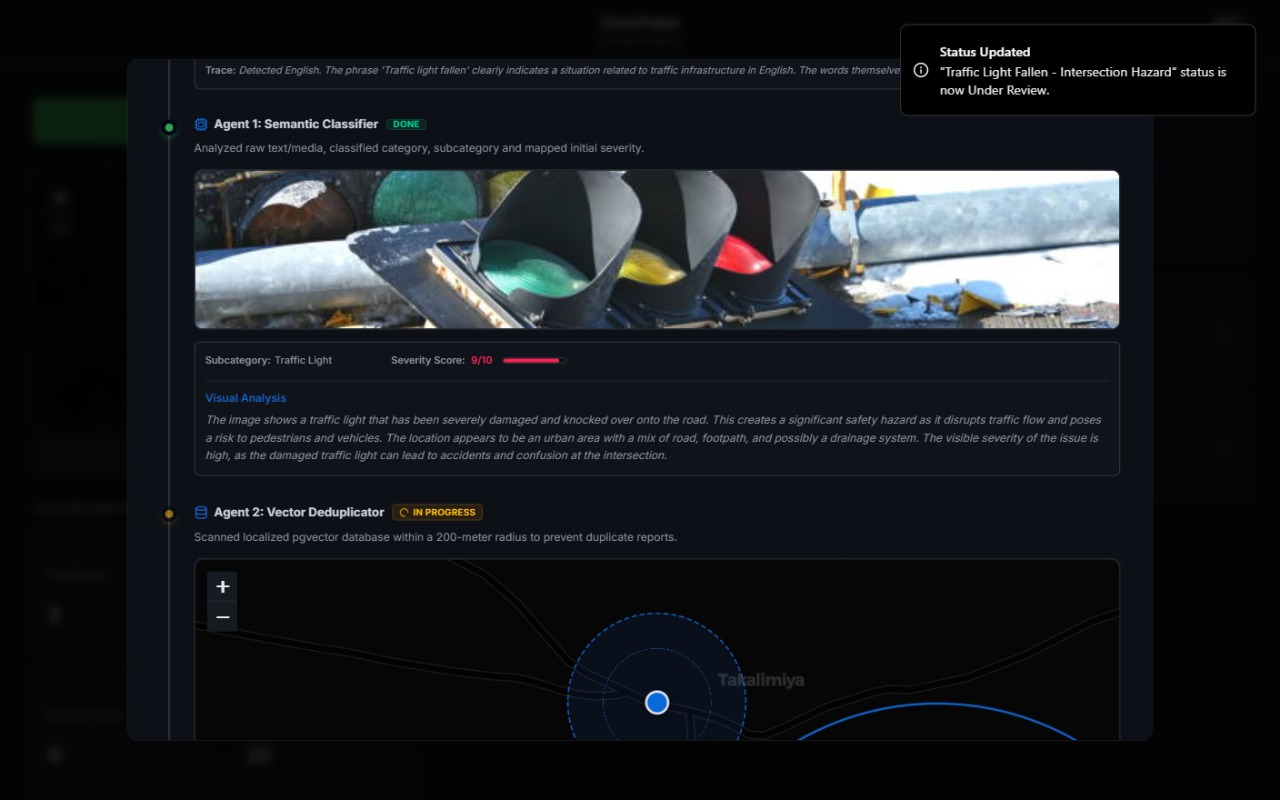
\includegraphics[width=\linewidth]{s6_issue_detail_3.jpg}
  \caption{Pipeline 3}
\end{subfigure}\hfill
\begin{subfigure}[t]{0.45\linewidth}
  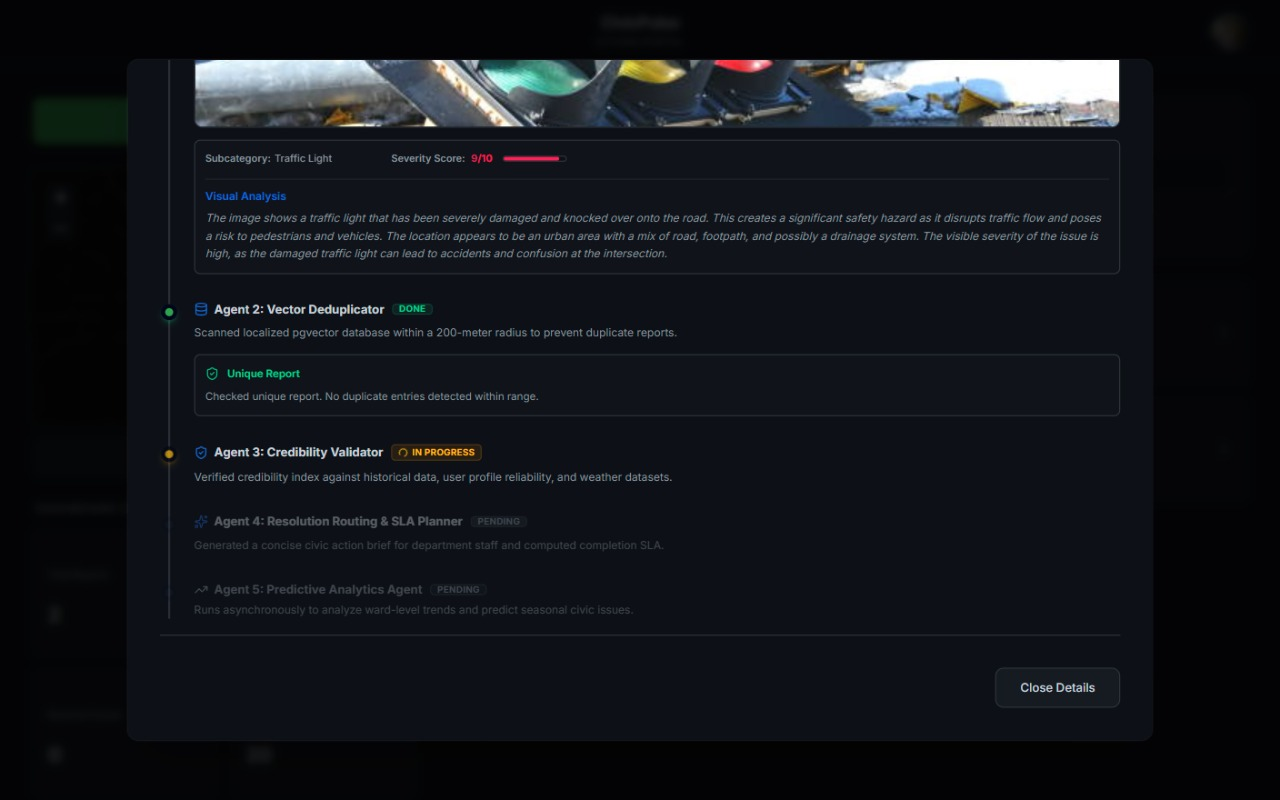
\includegraphics[width=\linewidth]{s6_issue_detail_4.jpg}
  \caption{Pipeline 4}
\end{subfigure}
\caption{Issue detail — full pipeline view from initial report to predictive analytics}
\end{figure}

\clearpage

\screenshot[0.85\linewidth]{s7_community_review.jpg}{Community verification — verify/deny panel}

\screenshot[0.85\linewidth]{s8_admin_inbox.jpg}{Admin dashboard — issue inbox with filters}

\clearpage

\screenshot[0.85\linewidth]{s9_admin_map.jpg}{Admin map — India-wide issue clusters}

\screenshot[0.85\linewidth]{s10_agent5.jpg}{Agent 5 predictive alerts panel}

\clearpage

\screenshot[0.85\linewidth]{s11_route_planner.jpg}{Route Planner — cluster selection + TSP route}

\screenshot[0.85\linewidth]{s12_agent2_map.jpg}{Agent 2 deduplication map — cluster visualisation}

\clearpage

\clearpage

% ============================================================
\section{User Perspective — Accessibility and Inclusivity}
\label{sec:ux}
% ============================================================

\subsection{Non-English Speaker User Story}

Consider \textbf{Sunita}, a homemaker in Nashik who writes only in Marathi:

\begin{enumerate}
  \item \textbf{Login:} Opens the app, taps ``Citizen,'' signs in with Google (consent screen renders in her device language). No English required.
  \item \textbf{Reporting:} She sees a burst water pipe. She opens the Report page and \textit{types} in Marathi: ``\textbf{\marathifont माझ्या गल्लीत पाण्याची पाइप फुटली आहे, पाणी वाहत आहे.}'' She taps the webcam button to attach a photo and hits ``Use GPS.''
  \item \textbf{Agent 0:} Detects Marathi, translates to English: ``A water pipe has burst in my lane, water is flowing.'' Translation trace stored.
  \item \textbf{Agents 1–4:} Classify as utility/water\_leakage, severity 7, department: Water Supply. Deduplication passes. Credibility 9/10 (photo + GPS). Civic brief generated in both English and Marathi.
  \item \textbf{Dashboard:} Sunita's \tech{local\_civic\_brief} is displayed in Marathi — she reads the municipality's action plan in her own language.
  \item \textbf{Resolution:} Pipe fixed → +50 karma → shareable Impact Receipt for WhatsApp.
\end{enumerate}

\subsection{Accessibility Features}

\begin{tabular}{@{} L{5.5cm} L{8.5cm} @{}}
\toprule
\rowcolor{cpblue}
\thead{Feature} & \thead{Benefit} \\
\midrule
Type in any language            & Agent 0 automatically translates; no English required \\
Voice input (English)           & Citizens can speak in English; text is transcribed by the browser's Web Speech API \\
Localised civic brief           & Resolution summaries in the citizen's own language \\
GPS auto-detection              & No need to type an address \\
Webcam capture                  & No separate camera app needed \\
Drag-and-drop upload            & Intuitive on all devices \\
Real-time pipeline tracking     & Citizens know exactly what is happening \\
Mobile-first layout             & Fully usable on any smartphone \\
Dark OLED mode                  & Reduces battery drain on AMOLED screens \\
Keyboard navigation (Radix)     & Full keyboard + screen reader support \\
\bottomrule
\end{tabular}

\clearpage

% ============================================================
\section{Technical Implementation}
\label{sec:technical}
% ============================================================

\subsection{Unified AI Client}
\textbf{File:} \file{lib/ai/client.ts} (318 lines)

Single point of contact for all AI operations with four exported functions:

\begin{tabular}{@{} L{5.5cm} L{4cm} L{4cm} @{}}
\toprule
\rowcolor{cpblue}
\thead{Function} & \thead{Purpose} & \thead{Used By} \\
\midrule
\tech{generateStructuredJSON<T>(...)} & Typed JSON from LLM & All 6 agents \\
\tech{analyzeImage(url, prompt)} & Multimodal vision & Agent 1 \\
\tech{generateEmbedding(text)} & 768-dim embedding & Submission, Agent 2 \\
\tech{generateText(prompt, system?)} & Plain text & Utility \\
\bottomrule
\end{tabular}

\textbf{Key implementation details:} Singleton pattern for client instances; custom \tech{fetch} with \tech{keepalive: false} to prevent \tech{UND\_ERR\_SOCKET} behind tunnels; JSON parsing strips markdown fences before \tech{JSON.parse()}.

\subsection{Three Supabase Clients}

\begin{tabular}{@{} L{4.5cm} L{4cm} L{5.5cm} @{}}
\toprule
\rowcolor{cpblue}
\thead{Client} & \thead{Auth Level} & \thead{Usage} \\
\midrule
\tech{createClient()} & Anon key (RLS) & Browser components \\
\tech{createServerSupabaseClient()} & Anon + cookie session & Server components, API routes \\
\tech{createServiceClient()} & Service role (RLS bypassed) & Agent pipeline (no user session) \\
\bottomrule
\end{tabular}

\subsection{Auth Flow}
The OAuth flow: Google consent → callback \file{/auth/callback} → \tech{exchangeCodeForSession()} → role-based redirect. The \tech{role=admin} query parameter in the redirect URL sets the user's profile role and sends them to \file{/admin/dashboard}.

Auth middleware (\file{proxy.ts}) protects \file{/dashboard}, \file{/report}, and \file{/admin}. For \file{/admin} paths, it additionally queries the \tech{profiles} table to verify \tech{role='admin'}.

\subsection{Community Verification System}
\textbf{Files:} \file{app/api/reviews/route.ts}, \file{app/api/reviews/[issueId]/vote/route.ts}

\begin{enumerate}
  \item \textbf{Fetch reviewable issues:} PostGIS \tech{ST\_DWithin} within 1 km of the user's saved home location; excludes their own reports and already-voted issues.
  \item \textbf{Cast vote:} Records verdict, awards +2 karma, checks quorum (min 3 votes).
  \item \textbf{Quorum resolution:} Confirm majority → auto-resume pipeline at Agent 4 (\file{/api/reports/retry}). Deny majority → close issue, --5 karma to reporter.
\end{enumerate}

\subsection{PostGIS WKB Decoding}
Supabase returns geography columns as hex-encoded WKB. Four routes decode via \tech{wkx}: \tech{wkx.Geometry.parse(Buffer.from(hex, 'hex')).toGeoJSON()}, extracting \tech{coordinates[1]} (lat) and \tech{coordinates[0]} (lng). WKT text format handled as fallback.



\clearpage

% ============================================================
\section{Database Schema}
\label{sec:db}
% ============================================================

\subsection{Entity Relationship Diagram}

\begin{figure}[H]
\centering
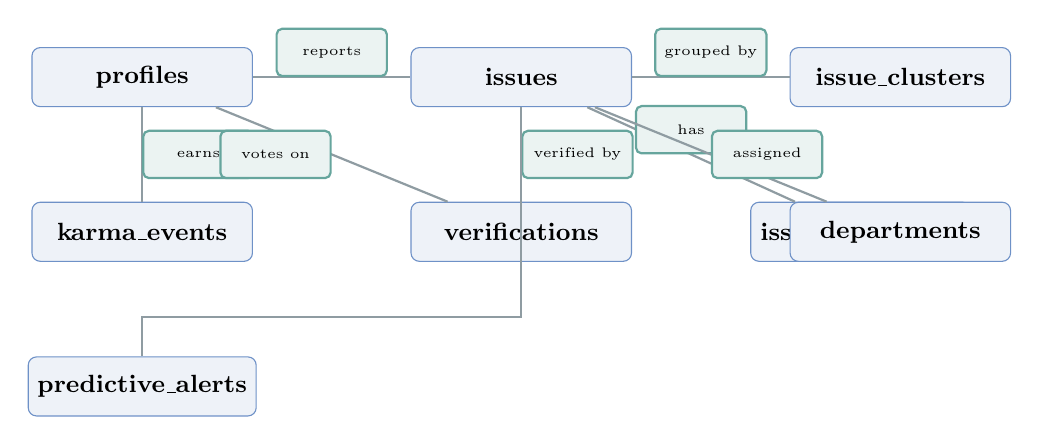
\begin{tikzpicture}[
  entity/.style={draw=cpblue!60, fill=cpblue!7, rounded corners=3pt,
                 minimum height=0.75cm, minimum width=2.8cm, align=center, font=\small\bfseries},
  rel/.style={draw=cpteal!60, fill=cpteal!8, rounded corners=2pt,
              minimum height=0.6cm, minimum width=1.4cm, align=center, font=\tiny},
  line/.style={draw=cpgray!60, thick},
  node distance=1.2cm and 1.5cm
]
% Entities
\node[entity] (profiles)  {profiles};
\node[entity, right=2cm of profiles] (issues) {issues};
\node[entity, right=2cm of issues] (clusters) {issue\_clusters};
\node[entity, below=1.2cm of issues] (verif) {verifications};
\node[entity, below=1.2cm of profiles] (karma) {karma\_events};
\node[entity, right=1.5cm of verif] (comments) {issue\_comments};
\node[entity, below=1.2cm of clusters] (depts) {departments};
\node[entity, below=1.2cm of karma] (alerts) {predictive\_alerts};

% Relations
\draw[line] (profiles) -- node[rel,above]{reports} (issues);
\draw[line] (issues) -- node[rel,above]{grouped by} (clusters);
\draw[line] (profiles) -- node[rel,right]{earns} (karma);
\draw[line] (issues) -- node[rel,right]{verified by} (verif);
\draw[line] (issues) -- node[rel,above]{has} (comments);
\draw[line] (depts) -- node[rel,right]{assigned} (issues);
\draw[line] (profiles) -- node[rel,left]{votes on} (verif);
\draw[line] (alerts.north) -- ++(0,0.5) -| (issues.south);
\end{tikzpicture}
\caption{Database entity relationships — 7 tables with PostGIS geography and pgvector extensions}
\end{figure}

\subsection{Key SQL RPC Functions}

\begin{tabular}{@{} L{5.5cm} L{8.5cm} @{}}
\toprule
\rowcolor{cpblue}
\thead{Function} & \thead{Purpose} \\
\midrule
\tech{match\_issues(embedding, threshold, count)} & pgvector cosine similarity search — returns top N issues above threshold \\
\tech{issues\_within\_radius(lat, lng, radius, category)} & PostGIS \tech{ST\_DWithin} — spatial proximity search \\
\tech{increment\_cluster\_count(cluster\_id)} & Atomic cluster size counter \\
\bottomrule
\end{tabular}

\clearpage

% ============================================================
\section{DevOps, CI/CD, and Cloud Deployment}
\label{sec:devops}
% ============================================================

\begin{importantbox}
\textbf{Live deployment:} \href{https://civicpulse-948264080742.asia-south1.run.app}{\tech{https://civicpulse-948264080742.asia-south1.run.app}}
\end{importantbox}

\subsection{CI/CD Pipeline}

\begin{figure}[H]
\centering
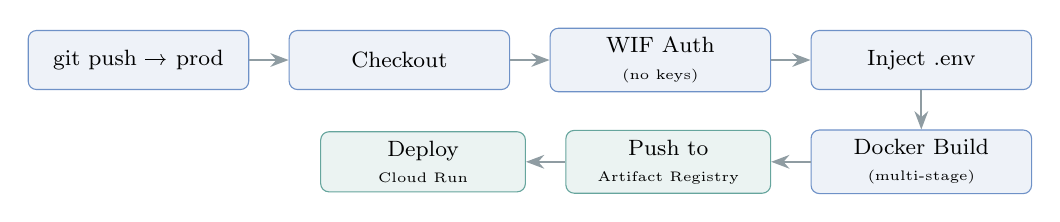
\begin{tikzpicture}[
  stepbox/.style={rounded corners=3pt, draw=cpblue!60, fill=cpblue!7,
               minimum height=0.75cm, minimum width=2.8cm, align=center, font=\footnotesize},
  cloud/.style={rounded corners=3pt, draw=cpteal!60, fill=cpteal!8,
                minimum height=0.75cm, minimum width=2.6cm, align=center, font=\footnotesize},
  arr/.style={-Stealth, thick, cpgray!60},
  node distance=0.45cm
]
\node[stepbox] (push) {git push → prod};
\node[stepbox, right=0.5cm of push] (checkout) {Checkout};
\node[stepbox, right=0.5cm of checkout] (auth) {WIF Auth\\\tiny(no keys)};
\node[stepbox, right=0.5cm of auth] (env) {Inject .env};
\node[stepbox, below=0.5cm of env] (build) {Docker Build\\\tiny(multi-stage)};
\node[cloud, left=0.5cm of build] (push2) {Push to\\\tiny Artifact Registry};
\node[cloud, left=0.5cm of push2] (deploy) {Deploy\\\tiny Cloud Run};

\draw[arr] (push)--(checkout); \draw[arr] (checkout)--(auth);
\draw[arr] (auth)--(env); \draw[arr] (env)--(build);
\draw[arr] (build)--(push2); \draw[arr] (push2)--(deploy);
\end{tikzpicture}
\caption{GitHub Actions CI/CD: push to \texttt{prod} → WIF auth → Docker build → Artifact Registry → Cloud Run}
\end{figure}

\textbf{Trigger:} Push to the \tech{prod} branch.\\
\textbf{Auth:} \tech{google-github-actions/auth@v2} with Workload Identity Federation — no service account JSON anywhere.\\
\textbf{Docker build:} Passes all \tech{NEXT\_PUBLIC\_*} vars as build args (Next.js inlines these at build time).\\
\textbf{Deploy:} \tech{google-github-actions/deploy-cloudrun@v2} with \tech{--allow-unauthenticated}.

\subsection{Multi-Stage Dockerfile}

\begin{tabular}{@{} L{2cm} L{3.5cm} L{8.5cm} @{}}
\toprule
\rowcolor{cpblue}
\thead{Stage} & \thead{Base Image} & \thead{Purpose} \\
\midrule
\tech{deps}    & \tech{node:20-alpine} & Install Bun, run \tech{bun install --frozen-lockfile} \\
\tech{builder} & \tech{node:20-alpine} & Copy source, set \tech{NEXT\_PUBLIC\_*} build args, run \tech{bun run build} \\
\tech{runner}  & \tech{node:20-alpine} & Non-root user (\tech{nextjs:1001}), copy standalone output, pre-install \tech{sharp} \\
\bottomrule
\end{tabular}

\clearpage

% ============================================================
\section{Completeness and Usability}
\label{sec:completeness}
% ============================================================

\subsection{End-to-End Citizen Flow}

\begin{tabular}{@{} C{0.6cm} L{4cm} L{9.4cm} @{}}
\toprule
\rowcolor{cpblue}
\thead{\#} & \thead{Feature} & \thead{Implementation} \\
\midrule
1 & Authenticate         & Google OAuth or email magic link via Supabase Auth \\
2 & Report issue         & Text (any language), photo/video (file, drag-drop, webcam), voice (English), GPS or map picker \\
3 & Track processing     & Real-time pipeline stage updates via Supabase Realtime \\
4 & View results         & Category, severity, civic brief (English + local language), SLA deadline, department \\
5 & Community verify     & View nearby low-credibility issues; cast verify/deny votes with comments \\
6 & Earn karma           & Points for reporting, reviewing, getting confirmed, issue resolved \\
7 & Leaderboard          & Top 10 citizens by karma; personal rank displayed \\
8 & Impact Receipt       & Shareable OG image for social media \\
9 & Retry failed         & Pipeline auto-resumes from last successful agent \\
\bottomrule
\end{tabular}

\subsection{End-to-End Admin Flow}

\begin{tabular}{@{} C{0.6cm} L{4cm} L{9.4cm} @{}}
\toprule
\rowcolor{cpblue}
\thead{\#} & \thead{Feature} & \thead{Implementation} \\
\midrule
1 & Admin login          & Google OAuth with \tech{role=admin} parameter \\
2 & Issue inbox          & Filterable issue list with real-time updates \\
3 & Manage issues        & Status updates, department assignment, comment thread \\
4 & Map view             & Mapbox issue pins with geographic DBSCAN cluster circles \\
5 & Predictive analysis  & Agent 5 with configurable lookback; heatmap overlay \\
6 & Route optimisation   & TSP routing for field teams via Google Maps Routes API \\
\bottomrule
\end{tabular}



\subsection{Test Coverage}
Twelve dedicated test files in \file{tests/}: agents 1–4, DB connectivity, geolocation, Gemini vision, Ollama vision, update operations, community voting, and pipeline retry.

\clearpage

% ============================================================
\section{What Makes CivicPulse Different}
\label{sec:diff}
% ============================================================

\begin{longtable}{@{} L{4cm} L{3.5cm} L{3.5cm} L{3cm} @{}}
\toprule
\rowcolor{cpblue}
\thead{Feature} & \thead{Municipal Portals} & \thead{311 Apps (US)} & \thead{CivicPulse} \\
\midrule
\endhead
AI classification        & \textbf{\color{cpgray}--}              & Keyword matching    & \textbf{6-agent LangGraph + Gemini} \\
Duplicate detection      & \textbf{\color{cpgray}--}              & Text matching only  & \textbf{Vector + spatial + AI} \\
Multilingual (typed)     & Separate portals & English only       & \textbf{Auto-detect + translate} \\
Predictive analytics     & \textbf{\color{cpgray}--}              & \textbf{\color{cpgray}--}                  & \textbf{Geographic DBSCAN + Gemini Pro} \\
Community verification   & \textbf{\color{cpgray}--}              & \textbf{\color{cpgray}--}                  & \textbf{Quorum-based + karma} \\
Real-time tracking       & Email only      & Push notifications  & \textbf{Supabase Realtime} \\
Route optimisation       & \textbf{\color{cpgray}--}              & \textbf{\color{cpgray}--}                  & \textbf{Google Maps TSP} \\
Mobile-first design      & Rarely          & Some                & \textbf{Full mobile-first + OLED} \\
\bottomrule
\end{longtable}

\section{Future Roadmap}
\label{sec:roadmap}

\begin{tabular}{@{} L{2cm} L{4cm} L{8cm} @{}}
\toprule
\rowcolor{cpblue}
\thead{Priority} & \thead{Feature} & \thead{Description} \\
\midrule
High   & WhatsApp Integration      & Citizens report via WhatsApp (text+photo+location) → same pipeline via webhook \\
High   & Web Push Notifications    & Infrastructure already in place (VAPID keys, push\_subscription column) \\
Medium & Scheduled Agent 5         & Cloud Run scheduled job (cron) instead of manual admin trigger \\
Medium & Ward-Level Analytics      & Resolution rates, SLA compliance, issue distribution by municipal ward \\
Low    & False Closure Detection   & Citizens challenge ``resolved'' status if issue persists \\
Low    & Multi-City Support        & Configuration-driven city selection with per-city department databases \\
\bottomrule
\end{tabular}

\clearpage

% ============================================================
\section{File Reference}
\label{sec:files}
% ============================================================

\subsection{Application Pages}

\begin{tabular}{@{} L{6cm} C{1cm} L{7cm} @{}}
\toprule
\rowcolor{cpblue}
\thead{File} & \thead{Lines} & \thead{Purpose} \\
\midrule
\file{app/layout.tsx}                        & 26  & Root layout: Inter, dark mode, Toaster \\
\file{app/page.tsx}                          & 32  & Landing: role selection, auth redirect \\
\file{app/auth/login/page.tsx}               & 126 & Login UI: Google + email magic link \\
\file{app/auth/callback/route.ts}            & 28  & OAuth code exchange, role-based redirect \\
\file{app/report/page.tsx}                   & 563 & Report: text, voice, image, video, GPS, map \\
\file{app/dashboard/page.tsx}                & 39  & Citizen dashboard server component \\
\file{app/admin/dashboard/page.tsx}          & 40  & Admin dashboard server component \\
\file{app/receipt/[issue\_id]/route.tsx}     & 118 & OG Impact Receipt (1200×630, edge runtime) \\
\bottomrule
\end{tabular}

\subsection{API Routes}

\begin{tabular}{@{} L{7cm} C{1cm} L{6cm} @{}}
\toprule
\rowcolor{cpblue}
\thead{File} & \thead{Lines} & \thead{Purpose} \\
\midrule
\file{api/reports/process/route.ts}          & 88  & Pipeline entry: insert + embed + run \\
\file{api/reports/retry/route.ts}            & 109 & Resume failed pipeline \\
\file{api/issues/map/route.ts}               & 52  & All issues with decoded WKB locations \\
\file{api/reviews/route.ts}                  & 162 & Community-reviewable issues within 1 km \\
\file{api/reviews/[issueId]/vote/route.ts}   & 147 & Cast vote, quorum, auto-resume \\
\file{api/admin/clusters/route.ts}           & 81  & Geographic DBSCAN clusters for admin map \\
\file{api/admin/predictive/run/route.ts}     & 43  & Trigger Agent 5 \\
\file{api/admin/routes/optimize/route.ts}    & 89  & Google Maps Routes TSP \\
\file{api/leaderboard/route.ts}              & 80  & Top 10 citizens by karma \\
\bottomrule
\end{tabular}

\subsection{Agent and Library Files}

\begin{tabular}{@{} L{6.5cm} C{1cm} L{6.5cm} @{}}
\toprule
\rowcolor{cpblue}
\thead{File} & \thead{Lines} & \thead{Purpose} \\
\midrule
\file{lib/ai/client.ts}                       & 318 & Unified AI: Gemini + Ollama, 4 functions \\
\file{lib/agents/agent0-translation.ts}        & 79  & Language detection + translation \\
\file{lib/agents/agent1-classifier.ts}         & 100 & Multimodal classification \\
\file{lib/agents/agent2-deduplication.ts}      & 178 & Three-layer deduplication \\
\file{lib/agents/agent3-validation.ts}         & 161 & Weather-aware credibility scoring \\
\file{lib/agents/agent4-resolution.ts}         & 140 & Civic brief + SLA computation \\
\file{lib/agents/agent5-predictive.ts}         & 158 & Geographic DBSCAN + Gemini Pro \\
\file{lib/agents/pipeline.ts}                  & 124 & LangGraph StateGraph wiring \\
\file{lib/utils/clustering.ts}                 & 174 & Geographic DBSCAN (Haversine, 50 km cap) \\
\file{proxy.ts}                                & 57  & Auth middleware: route + role protection \\
\bottomrule
\end{tabular}

% ── BACK COVER / CLOSING ─────────────────────────────────────
\vspace*{\fill}
\begin{center}
\begin{tcolorbox}[
  enhanced, colback=cpblue!4, colframe=cpblue!8,
  boxrule=0.5pt, arc=6pt,
  left=15pt, right=15pt, top=12pt, bottom=12pt,
  width=0.85\linewidth,
  drop shadow={shadow xshift=0mm, shadow yshift=-1mm, opacity=0.15}
]
\centering
{\sffamily\bfseries\color{cpblue}\large CivicPulse}\\[4pt]
{\sffamily\color{cpgray}\small Problem Statement 2: Community Hero — Hyperlocal Problem Solver}\\[10pt]
{\color{cpteal}\rule{0.4\linewidth}{0.8pt}}\\[10pt]
{\sffamily\footnotesize\color{cpgray}Submitted by \textbf{Ronit Sonawane} · B.Tech CSE, IIT Guwahati}\\[2pt]
{\sffamily\scriptsize\color{cpgray!80}\href{https://github.com/ronits2407/civicpulse}{github.com/ronits2407/civicpulse} \quad |\quad June 2026}
\end{tcolorbox}
\end{center}

\end{document}
